%!TEX root = restart.tex
\section{Preliminaries\label{sec:Preliminaries}}


\subsection{Conservation law PDEs\label{sub:Hyperbolic-PDE's}}

In this paper we focus on scalar hyperbolic conservation laws. In particular, we consider the non-linear transport equation of the form:
\begin{equation}
	\partial_t\cvar\left(t,x\right)+\partial_x f\left(\cvar\left(t,x\right)\right)=0 \quad (t,x) \in \R^+ \times \R\label{eq:cons}
\end{equation}
where $\cvar=\cvar(t,x) \in \; \R^+$ is the scalar conserved quantity and $f:\R^+\rightarrow \R^+$ is the flux function. Throughout the article we suppose that $f$ is a stricly concave function. \\
The Cauchy problem to solve is then 
\begin{equation}
	\label{eq:CP}
	\left\{
	\begin{array}{ll}
		\partial_t \cvar+ \partial_x f(\cvar) =0, & (t,x)\in\R^+\times \R, \\
		\cvar(0,x)=\initstate(x),                 & x \in \R               \\
	\end{array}
	\right.
\end{equation}
where $\initstate(x)$ is the initial condition.
It can be shown that there exists a unique weak entropy solution for the Cauchy problem \eqref{eq:CP} as described in Definition \ref{def:weak-sol}. 
\begin{defn}\label{def:weak-sol}
	A function $\cvar \in \; \mathcal{C}^0(\R^+; \mathbf{L}^1_{loc}\cap \mathbf{BV})$ is an admissible solution to \eqref{eq:CP} if
	\begin{itemize}
		\item $\cvar$ is a weak solution, i.e., $\cvar : \R^+\times\R\rightarrow \R^+$ such that
		\begin{equation}	
			\int_{\R^+}\int_{\R}\Big( \cvar \partial_t\varphi +f(\cvar)\partial_x\varphi \Big)dxdt=0, 
		\end{equation}
		for every $\varphi \in \mathbf{C}^1_c(\R^+\times \R; \R).$
		\item $\cvar$ satisfies the Kru\v{z}hkov entropy condition~\cite{Kruzkov1970} on $(\R^+\times\R)$, i.e.,for every $k\in \R$ and for all $\varphi \in \mathcal{C}^1_c(\R^+\times \R;\R^+),$
		\begin{eqnarray}
			\label{eq:kruzhkov}
			&\int_{\R^+}\int_{\R}(\modulo{\cvar -k}  \partial_t \varphi + \sgn{(\cvar-k }) (f(\cvar)-f(k))\partial_x\varphi)dxdt& \nonumber\\
			&+\int_{\R}\modulo{\initstate-k}\varphi(0,x)dx\geq 0.&
		\end{eqnarray} 
	\end{itemize}
\end{defn}
For further details regarding the theory of hyperbolic conservation laws we refer the reader to~\cite{garavello2006traffic,Evans1998}.

%We are mainly interested in scalar hyperbolic conservation laws of
%the following form:
%
%\begin{equation}
%\pfrac{\cvar\left(t,x\right)}t+\pfrac{f\left(\cvar\left(t,x\right)\right)}x=0\label{eq:cons}
%\end{equation}
%where $\cvar:\left[0,\infty\right)\times\mathbb{R}\rightarrow\mathbb{R}$
%is the scalar ``conserved'' quantity, and $f:\mathbb{R}\rightarrow\mathbb{R}$
%is the flux function. If we assume $f$ to be $C^{2}$, we can rewrite
%Equation~(\eqref{eq:cons}) as:
%
%\begin{equation}
%\cvar_{t}+f\left(\cvar\right)_{x}=0\label{eq:cons-smooth}
%\end{equation}
%
%
%For a particular initial condition $\initstate\in BV\cap L_{\text{loc}}^{1}\left(\mathbb{R};\mathbb{R}\right)$,
%we seek ``weak'' solutions of $\cvar$ for the Cauchy problem:
%
%\begin{equation}
%\begin{cases}
%\cvar_{t}+f\left(\cvar\right)_{x} & =0\\
%\cvar\left(0,x\right) & =\initstate\left(x\right)
%\end{cases}\label{eq:cauchy}
%\end{equation}
%More details on weak solutions to hyperbolic PDEs are available, in
%particular, in~\cite{garavello2006traffic,Evans1998}. It can be
%shown that there exists a unique weak solution exists to a Cauchy
%problem of the form in~\eqref{eq:cauchy}.
\begin{defn}
	\label{def:Riemann-Problem}Riemann Problem.
	
	A Riemann problem is a Cauchy problem with a piecewise-constant initial data (called the Riemann data):
	
	\[
		\initstate(x)=\begin{cases}
		\cvar_{-} & x<0\\
		\cvar_{+} & x\ge 0
		\end{cases}
	\]
	%with one point of discontinuity, $x=\bar{x}$. Without loss of generality,
	%we may take $\bar{x}=0$.
\end{defn}
%It can be shown that the $\cvar$ solution generated from the Riemann
%data $\left(\cvar_{-};\cvar_{+}\right)$ has a constant value along
%lines of constant $\frac{x}{t}$. 
We denote the self-similar entropy weak solutions between $\cvar_{-}$ and $\cvar_{+}$ by $\ss{\frac{x}{t}}{\cvar_{-}}{\cvar_{+}}$.


\subsection{Network of PDEs\label{sub:Network-of-PDE's}}

A network
% of hyperbolic conservation laws such as~(\eqref{eq:cons})
is defined as a set of $\nlinks$ links $\links=\intrange 1{\nlinks}$,
with junctions $\jns$. Each junction $\jn\in\jns$ is defined
as the union of  two non-empty sets: the set of $\ninc_{\jn}$ incoming links $\Inc\left(\jn\right)=\tuple{\jlink{\jn}1}{\jlink{\jn}{\ninc_{\jn}}}\subset\links$
and the set of $\nout_{\jn}$ outgoing links $\Out\left(\jn\right)=\tuple{\jlink{\jn}{\ninc_{\jn}+1}}{\jlink{\jn}{\ninc_{\jn}+\nout_{\jn}}}\subset\links$.
Each link $\link\in\links$ has an associated upstream junction $\jup{\link}\in\jns$
and downstream junction $\jdown{\link}\in\jns$, and has an associated
spatial domain $\left(0,L_{\link}\right)$ over which the evolution
of the state on link $\link$, $\cvar_{\link}\left(t,x\right)$, solves
the Cauchy problem:

\begin{equation}
	\begin{cases}
		\left(\cvar_{\link}\right)_{t}+f\left(\cvar_{\link}\right)_{x} & =0                                \\
		\cvar_{\link}\left(0,x\right)                                  & =\initstate_{\link}\left(x\right) 
	\end{cases}\label{eq:cauchy-i}
\end{equation}
where $\initstate_{\link}\in BV\cap L_{\text{loc}}^{1}\left(\mathbb{R};\mathbb{R}\right)$
is the initial condition on link $\link$. For simplicity of notation,
this section considers a single junction $\jn\in\jns$ with $\Inc\left(\jn\right)=\left(1,\ldots,\ninc\right)$
and $\Out\left(\jn\right)=\left(\ninc+1,\ldots,\ninc+\nout\right)$.
\begin{rem}
	There is redundancy in the labeling of the junctions, for if link
	$i$ is directly upstream of link $j$, then we have $\jdown{\link}=\jup j$.
	See Figure~\ref{fig:Space-discretization-for}.
\end{rem}
While the dynamics on each link $\cvar_{\link}\left(t,x\right)$ is
determined by~\eqref{eq:CP}, the dynamics at junctions
still needs to be defined.
\begin{defn}
	Riemann problem at junctions. 
	
	A Riemann problem at $\jn$ is a Cauchy problem corresponding to an initial data $\tuple{\initstate_{1}}{\initstate_{\ninc+\nout}}\in\mathbb{R}^{\ninc+\nout}$ which is constant on each link $\link$ .
	
	%Let all links $\link$ have a constant initial profile $\cvar_{\link}\left(0,x\right)=\initstate_{\link}\in\mathbb{R}$
	%(called the Riemann data) with incoming links having a spatial domain
	%$\left(-\infty,0\right)$ and outgoing links having a spatial domain
	%$\left(0,\infty\right)$. The solution of $\cvar_{\link}\left(x,t\right)$
	%for all links $\link\in\Inc\left(\jn\right)\cup\Out\left(\jn\right)$
	%and $t\ge0$ is defined as the solution to the Riemann problem at
	%junction $J$ with initial data $\tuple{\initstate_{1}}{\initstate_{\ninc+\nout}}\in\mathbb{R}^{\ninc+\nout}$.
\end{defn}
\begin{defn}
	A Riemann solver is a map that assigns a solution to each Riemann initial data. For each junction $\jn$ it is a function
	
	\begin{eqnarray*}
		\RS: & \mathbb{R}^{m+n} & \rightarrow\mathbb{R}^{m+n}\\
		& \tuple{\initstate_{1}}{\initstate_{\ninc+\nout}} & \mapsto\RS\tuple{\initstate_{1}}{\initstate_{\ninc+\nout}}=\tuple{\trace{\cvar}_{1}}{\trace{\cvar}_{\ninc+\nout}}
	\end{eqnarray*}
	where $\trace{\cvar}_{\link}$ provides the trace for link $\link$
	at the junction for all time $t\ge0$.
	
\end{defn}
For a link $i\in\Inc\left(\jn\right)$,
the solution $\cvar_{i}\left(t,x\right)$ over its spatial domain
$x<0$ is given by the solution to the following Riemann problem:

\begin{equation}
	\begin{cases}
		\left(\cvar_{\link}\right)_{t}+f\left(\cvar_{\link}\right)_{x} & =0             \\
		\cvar_{\link}\left(0,x\right)                                  & =\begin{cases} 
		\initstate_{\link}                                             & x<0            \\
		\trace{\cvar}_{\link}                                          & x\ge0,         
	\end{cases}
	\end{cases}\label{eq:riemann-problem}
\end{equation}
%which is essentially a Riemann problem with a ``virtual'' outgoing
%link, used to compute the solution of the junction problem in the
%incoming link near the junction.

The Riemann problem for an outgoing link is defined similarly, with
the exception that $\cvar_{\link}\left(0,x>0\right)=\initstate_{\link}$
and $\cvar_{\link}\left(0,x\le0\right)=\trace{\cvar}_{\link}$. Figure~\ref{fig:Solution-of-boundary}
gives a depiction of Riemann solution at the junction%
%\footnote{The assumption of an unbounded spatial domain is to eliminate the
%need to explicitly consider boundary conditions away from the junction,
%and for each link, the solution near the junction generalizes to the
%case when the spatial domain is bounded.%
%}. 
\begin{figure}
	\begin{centering}
		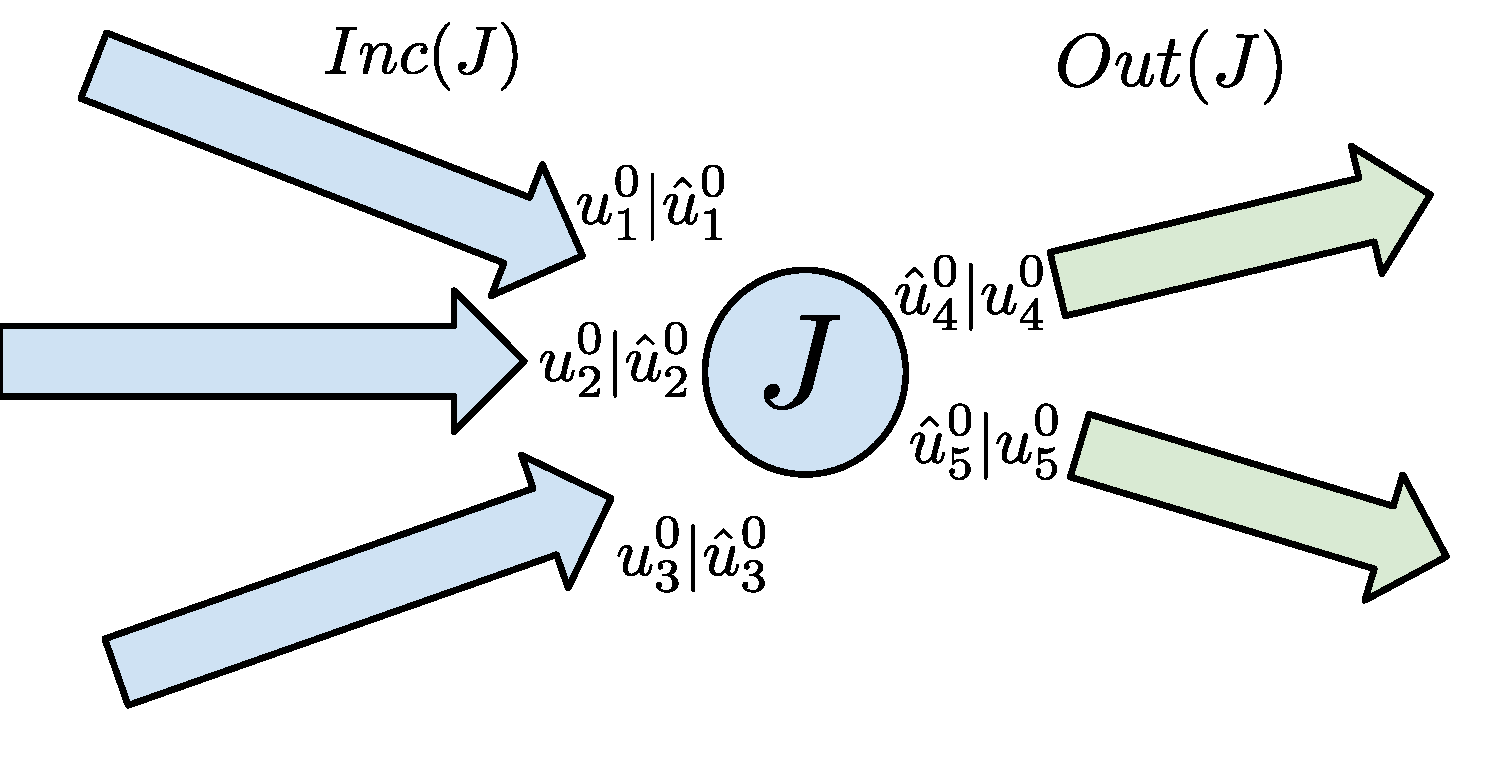
\includegraphics[width=0.5\columnwidth]{presentation/figs-gen/junctions-riemann-rs} 
		\par\end{centering}
		
		\caption{Solution of boundary conditions at junction. The boundary conditions
			$\tuple{\trace{\cvar}_{1}}{\trace{\cvar}_{5}}$ are produced by applying
			the Riemann solver to the initial conditions, $\tuple{\initstate_{1}}{\initstate_{5}}$.\label{fig:Solution-of-boundary}}
		\end{figure}
		
		
		Note that the following properties for the Riemann Solver holds:
		\begin{itemize}
			\item All waves produced from the solution to Riemann problems on all links,
			generated by the boundary conditions at a junction, must emanate out
			from the junction. Moreover, the solution to the Riemann problem
			on an incoming link must produce waves with negative speeds, while
			the solution on an outgoing link must produce waves with positive
			speed. 
			\item The sum of all incoming fluxes must equal the sum of all outgoing
			fluxes: 
			\[
				\sum_{i\in\Inc\left(\jn\right)}f\left(\trace{\cvar}_{\link}\right)=\sum_{j\in\Out\left(\jn\right)}f\left(\trace{\cvar}_{j}\right)
			\]
			This condition guarantees mass conservation at junctions.
			\item The Riemann solver must produce self-similar solutions, i.e. 
			\[
				\RS\left(\RS\tuple{\initstate_{1}}{\initstate_{\ninc+\nout}}\right)=\RS\tuple{\initstate_{1}}{\initstate_{\ninc+\nout}}=\tuple{\trace{\cvar}_{1}}{\trace{\cvar}_{\ninc+\nout}}
			\]
		\end{itemize}
		
		The justification for these conditions can be found in~\cite{garavello2006traffic}.
		
		
		\subsection{Godunov Discretization\label{sub:Godunov-Discretization}}
		
		In order to find approximate solutions we use the classical Godunov scheme~\cite{godunov1959}. We use the following notation: $x_{j+\frac{1}{2}}$ are the cell interfaces and   $t^{\tind}=k\Delta t$ the time with $\tind\in\mathbb{N}$ and $\xind\in\mathbb{Z}$. $x_{\xind}$ is the center of the cell, $\Delta x=x_{j+\frac{1}{2}}-x_{j-\frac{1}{2}}$ the cell width and $\Delta t$ is the time step. 
		\paragraph{Godunov scheme for a single link.}
		
		The Godunov scheme is based on the solutions of exact Riemann problems. The main idea of this method is to approximate the initial datum by a piecewise constant function, then the corresponding Riemann problems are solved exactly and a global solution is found by piecing them together. Finally one takes the mean on the cell and proceed by iteration. Given $\cvar(t,x),$ the cell average of $\cvar$ at time $t^{\tind}$ in the cell $C_{\xind}=]x_{j-\frac{1}{2}},x_{j+\frac{1}{2}}]$ is given by 
		\begin{equation}
			\discrete{\xind}{\tind}=\dfrac{1}{\Delta x}\int_{\xdis{\xind-\frac{1}{2}}}^{\xdis{\xind+\frac{1}{2}}}\dvar(t^{k},x)dx.\label{eq:godproj}
		\end{equation}
		Then we proceed as follows:
		\begin{enumerate}
			\item We solve the Riemann problem at each cell interface $x_{j+\frac{1}{2}}$ with initial data $(\dvar^{\tind}_{\xind-1},\dvar^{\tind}_{\xind}).$
			\item Compute the cell average at time $t^{\tind +1}$ in each computational cell and obtain $\dvar^{\tind +1}_{\xind}.$ 
		\end{enumerate}
		
		We remark that waves in two neighbouring cells do not intersect before $\Delta t$ if the following Courant\textendash{}Friedrichs\textendash{}Lewy (CFL) condition holds:
		\begin{equation}\label{eq:CFL}
			\lambda^{\max}\le\frac{\Delta x}{\Delta t},
		\end{equation}
		where $\lambda^{\max}=\underset{a}{\max}|f'\left(a\right)|$ is the maximum wave speed of the Riemann solution at the interfaces.\\
		Godunov scheme can be expressed as follows:
		\begin{equation}
			\discrete{\xind}{\tind+1}=\discrete{\xind}{\tind}-\frac{\Delta t}{\Delta x}(\god(\discrete{\xind}{\tind},\discrete{\xind+1}{\tind})-\god(\discrete{\xind-1}{\tind},\discrete{\xind}{\tind})),\label{eq:godscheme}
		\end{equation}
		where $g^{G}$ is the Godunov numerical flux given by
		
		\begin{eqnarray*}
			\god: & \mathbb{R}\times\mathbb{R} & \rightarrow\mathbb{R}\\
			& \left(\discrete{\xind}{},\discrete{\xind+1}{}\right) & \mapsto\god\left(\discrete{\xind}{},\discrete{\xind+1}{}\right)=f(W_{R}(0;\discrete{\xind}{},\discrete{\xind+1}{})).
		\end{eqnarray*}
		
		
		%To approximate a hyperbolic PDE of the form in~(\eqref{eq:cons-smooth})
		%with a discretization in both space and time, we use Godunov's scheme~\cite{godunov1959}.
		%Given an initial condition that is piecewise-constant, Godunov's scheme
		%gives a procedure to advance the system one time-step forward. Under
		%suitable stability conditions, this process can be repeated \emph{ad
		%infinum }by applying the scheme to the new condition generated from
		%the previous time-step.
		
		%We define a numerical grid using the following notations 
		%\begin{itemize}
		%\item $\Delta x$ is the fixed space grid size,
		%\item $\Delta t$ is the fixed time grid size, chosen with respect to the Courant\textendash{}Friedrichs\textendash{}Lewy (CFL) condition%
		%\footnote{This method can be generalized to non-uniform grid sizes, but is chosen
		%to be uniform to simplify notation%
		%}, 
		%\item $(t^{\tind},\xdis{\xind})=(k\Delta t,\xind\Delta x)$ for $\tind\in\mathbb{N}$
		%and $\xind\in\mathbb{Z}$ grid points%
		%\footnote{The CFL condition, $\lambda^{\max}\le\frac{\Delta x}{\Delta t}$,
		%guarantees that the waves in two neighboring cells do not interact
		%at the cell boundaries before $\Delta t$. Above $\lambda^{\max}=\underset{a}{\max}|f'\left(a\right)|$
		%is the maximum absolute wave speed. We assume henceforth that this
		%condition always holds for the chosen step sizes.%
		%}. For a link $\link\in\links$ with space domain $\left(0,\length_{\link}\right)$,
		%$\xind$ takes values in $\intrange 0{\length_{\link}^{\Delta}}$.
		%\end{itemize}
		%For a function $\dvar$ defined at the grid we write $\discrete{\xind}{\tind}=\dvar(t^{\tind},\xdis{\xind})$
		%for $\tind,\xind$ varying on a subset of $\mathbb{N}$ and $\mathbb{Z}$.
		%The space discretization scheme is depicted for a link $\link\in\links$
		%in Figure~\ref{fig:Space-discretization-for}
		\begin{figure}
			\begin{centering}
				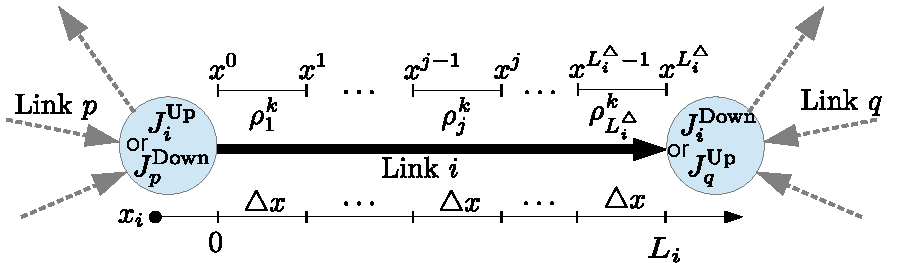
\includegraphics[width=0.6\columnwidth]{figs-gen/dx}
				\par\end{centering}
				
				\caption{Space discretization for a link $\link\in\links$. Step size $\Delta x$ is uniform with discrete value $\discrete{\xind}{\tind}$ representing
					the state between $x_{\xind-\frac{1}{2}}$ and $x_{\xind + \frac{1}{2}}$.\label{fig:Space-discretization-for}}
				
				
				\end{figure}
				
				%Consider a hyperbolic equation together with an initial condition
				%as expressed in~\eqref{eq:cauchy}. A solution of the discretized
				%problem is constructed by taking a piecewise constant approximation
				%of the initial data $\initvar{\dvar}^{\Delta}$ and then constructing
				%the solution iteratively from the approximate initial data as in~\eqref{eq:godproj}.
				%\begin{equation}
				%\discrete{\xind}{\tind}\approxeq\dfrac{1}{\Delta x}\int_{\xdis{\xind-\frac{1}{2}}}^{\xdis{\xind+\frac{1}{2}}}\dvar^{\Delta}(t^{k},x)dx.\label{eq:godproj}
				%\end{equation}
				%
				%
				%where $\cvar^{\Delta}\left(t,x\right)$ is an exact solution of~\eqref{eq:cauchy}
				%with initial condition $\initstate^{\Delta}$.
				%
				%Since $\cvar^{\Delta}$ in~\eqref{eq:godproj} is an exact solution
				%of~(\eqref{eq:cons-smooth}) we can use the Gauss-Green formula to
				%compute this value. Under the CFL condition, the solutions are locally
				%given by the solutions of the Riemann problems and, in particular,
				%the flux at $x=\xdis{\xind+\frac{1}{2}}$ for $t\in(t^{k},t^{k+1})$
				%is given by 
				%\[
				%f(\cvar(t,\xdis{\xind}))=f(W_{R}(0;\discrete{\xind}{\tind},\discrete{\xind+1}{\tind})).
				%\]
				%This flux solution is depicted in Figure~\ref{fig:Self-similar-solution-for}
				\begin{figure}
					\begin{centering}
						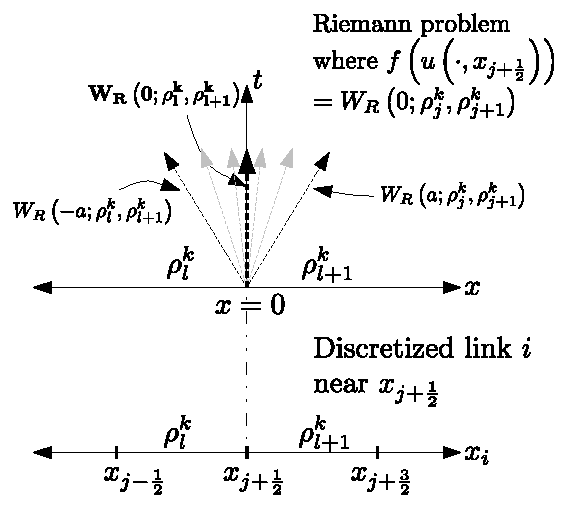
\includegraphics[width=0.5\columnwidth]{figs-gen/dx-to-riemann}
						\par\end{centering}
						
						\caption{Self-similar solution for Riemann problem with initial data $\left(\discrete{\xind}{\tind},\discrete{\xind+1}{\tind}\right)$.
							The self-similar solution at $\frac{x}{t}=0$ for the top diagram
							(i.e. $\ss 0{\discrete{\xind}{\tind}}{\discrete{\xind+1}{\tind}}$),
							gives the flux solution to the discretized problem in the bottom diagram.\label{fig:Self-similar-solution-for}}
						\end{figure}
						%.The flux at $x=\xdis{\xind-\frac{1}{2}}$ for $t\in(t^{k},t^{k+1})$
						%is given by 
						%\[
						%f(\cvar(t,\xdis{\xind-\frac{1}{2}}))=f(W_{R}(0;\discrete{\xind-1}{\tind},\discrete{\xind}{\tind})).
						%\]
						%As the flux is constant at $x=0$ for the Riemann problem, we can
						%put it out of the integral and, setting $\god(u,v)=f(W_{R}(0;u,v))$,
						%the scheme can be written as 
						%\begin{equation}
						%\discrete{\xind}{\tind+1}=\discrete{\xind}{\tind}-\frac{\Delta t}{\Delta x}(\god(\discrete{\xind}{\tind},\discrete{\xind+1}{\tind})-\god(\discrete{\xind-1}{\tind},\discrete{\xind}{\tind})),\label{eq:godscheme}
						%\end{equation}
						%where $g^{G}$ is the numerical flux:
						%
						%\begin{eqnarray*}
						%\god: & \mathbb{R}\times\mathbb{R} & \rightarrow\mathbb{R}\\
						% & \left(\discrete{\xind}{},\discrete{\xind+1}{}\right) & \mapsto\god\left(\discrete{\xind}{},\discrete{\xind+1}{}\right)=f(W_{R}(0;\discrete{\xind}{},\discrete{\xind+1}{}))
						%\end{eqnarray*}
						
						
						
						\paragraph{Godunov scheme at junctions.\label{par:Godunov-scheme-at}}
						
						The scheme just discussed applies to the case in which a single cell
						is adjacent to another single cell. Yet, at junctions, a cell may
						share a boundary with more than one cell. A more general Godunov flux
						can be derived for such cases. For incoming links near the junction,
						we have: 
						\begin{align*}
							\discrete{\length_{\link}^{\Delta}}{\tind+1}=\discrete{\length_{\link}^{\Delta}}{\tind}-\dfrac{\Delta t}{\Delta x}(f(\trace{\dvar}_{\length_{\link}^{\Delta}}^{\tind})-\god(\discrete{L_{i}^{\Delta}-1}{\tind},\discrete{L_{i}^{\Delta}}{\tind})), &   & \link\in\left\{ 1,\ldots,\ninc\right\} 
						\end{align*}
						where $\hat{\dvar}_{i}^{\tind}$ is the solution of the Riemann solver
						$\RS\tuple{\discrete 1{\tind}}{\discrete{\ninc+\nout}{\tind}}$ for
						link $\link$ at the junction. The same can be done for the outgoing
						links: 
						\begin{align*}
							\discrete 1{\tind+1}=\discrete 1{\tind}-\dfrac{\Delta t}{\Delta x}(\god(\discrete 1{\tind},\discrete 2{\tind})-f(\trace{\dvar}_{1}^{\tind})), &   & \link\in\left\{ \ninc+1,\ldots,\ninc+\nout\right\} 
						\end{align*}
						
						\begin{rem}
							Using the Godunov scheme, each mesh grid at a given $t^{\tind}$ can
							be seen as a node for a 1-to-1 junction with one incoming and one
							outgoing link. It is therefore more convenient to consider that every
							discretized cell is, rather, a link with both an upstream and downstream
							junction. Thus, we consider networks in which the state of each link
							$\link\in\links$ at a time-step $k\in\intrange 0{\ntime-1}$ is represented
							by the single discrete value $\discrete{\link}{\tind}$.
						\end{rem}
						The previous remark allows us to develop a generalized update step
						for all discrete state variables. We first introduce a definition
						in order to reduce the cumbersome nature of the preceding notation.
						Let the state variables adjacent to a junction $\jn\in\jns$ at a
						time-step $\tind\in\intrange 0{\ntime-1}$ be represented as $\juncstate{\jn}{\tind}\defeq\tuple{\discrete{\link_{\jn}^{1}}{\tind}}{\discrete{\link_{\jn}^{\ninc_{\jn}+\nout_{\jn}}}{\tind}}$.
						Similarly, we let the solution of a Riemann solver be represented
						as $\junctrace{\jn}{}\defeq\RS\left(\juncstate{\jn}{}\right)$. Then,
						for a link $\link\in\links$ with upstream and downstream junctions,
						$\jup{\link}$ and $\jdown{\link}$, and time-step $\tind\in\left\{ 0,\ldots,\ntime-1\right\} $,
						the update step becomes:
						
						\begin{align}
							\discrete{\link}{\tind+1} & =\discrete{\link}{\tind}-\dfrac{\Delta t}{\Delta x}\left(f\left(\left(\RS\left(\juncstate{\jdown{\link}}{\tind}\right)\right)_{\link}\right)-f\left(\left(\RS\left(\juncstate{\jup{\link}}{\tind}\right)\right)_{\link}\right)\right)\nonumber \\
							                          & =\discrete{\link}{\tind}-\dfrac{\Delta t}{\Delta x}\left(f\left(\left(\junctrace{\jdown{\link}}{}\right)_{\link}\right)-f\left(\left(\junctrace{\jup{\link}}{}\right)_{\link}\right)\right)\label{eq:reg-update}                               
						\end{align}
						
						
						where $\left(s\right)_{i}$ is the $i$th element of the tuple $s$.
						This equation is thus a general way of writing the Godunov scheme
						in a way which applies everywhere, including at junctions.
						
						
						\paragraph{Working directly with flux solutions at junctions.\label{par:Composing-the-Riemann}}
						
						The equations can be simplified if we do not explicitly represent
						the solution of the Riemann solver, $\junctrace{\jn}{}$, and, instead,
						directly calculate the flux solution from the Riemann data. We denote
						this direct computation by $\god_{\jn}$, the Godunov flux solution
						at a junction:
						
						\begin{eqnarray}
							\god_{\jn}: & \mathbb{R}^{\ninc_{\jn}+\nout_{\jn}} & \rightarrow\mathbb{R}^{\ninc_{\jn}+\nout_{\jn}}\nonumber \\
							& \juncstate{\jn}{} & \mapsto f\left(RS\left(\juncstate{\jn}{}\right)\right)=\left(f\left(\trace{\dvar}_{1}\right),\ldots,f\left(\trace{\dvar}_{\ninc+\nout}\right)\right)\label{eq:god-jn}
						\end{eqnarray}
						This gives a simplified expressions for the update step:
						
						\begin{equation}
							\discrete{\link}{\tind+1}=\discrete{\link}{\tind}-\dfrac{\Delta t}{\Delta x}\left(\left(\god_{\jdown{\link}}\left(\juncstate{\jdown{\link}}{\tind}\right)\right)_{\link}-\left(\god_{\jup{\link}}\left(\juncstate{\jup{\link}}{\tind}\right)\right)_{\link}\right)\label{eq:composed-flux}
						\end{equation}
						
						
						
						\paragraph{Full discrete solution method.\label{par:Full-solution-method}}
						
						We assume a discrete scalar hyperbolic network of PDEs with links
						$\links$ and junctions $\jns$, and a known discrete state at time-step
						$\tind$, $\left(\initdiscrete_{\link}^{\tind}:\link\in\links\right)$.
						The solution method for advancing the discrete system forward one
						time-step is given in Algorithm~(\ref{algo:rs-alg}), or alternatively
						Algorithm~(\ref{algo:god-alg}).
						
						\begin{algorithm}[H]
							\caption{\texttt{Riemann solver update procedure}}
							
							
							\lstinputlisting[basicstyle={\ttfamily\footnotesize},breaklines=true,label={algo:rs-alg},mathescape=true]{rs-alg}
						\end{algorithm}
						
						
						Algorithm~\ref{algo:rs-alg} takes as input the state at a time-step
						$\tind$ for all links $\left(\discrete{\link}{\tind}:\link\in\links\right)$
						and returns the state advanced by one time-step $\left(\discrete{\link}{\tind+1}:\link\in\links\right)$.
						The algorithm first iterates over all junctions $\jn$, calculating
						all the boundary conditions, $\junctrace{\jn}{\tind}$. Then, the
						algorithm iterates over all links $\link\in\links$ to compute the
						updated state $\discrete{\link}{\tind+1}$ using the previously computed
						boundary conditions, as in~\eqref{eq:reg-update}.
						
						\begin{algorithm}[h]
							\caption{\texttt{Godunov junction flux update procedure}}
							
							
							\lstinputlisting[basicstyle={\ttfamily\footnotesize},breaklines=true,label={algo:god-alg},mathescape=true]{god-alg}
						\end{algorithm}
						
						
						Algorithm~\ref{algo:god-alg} is similar to Algorithm~\ref{algo:rs-alg},
						except that the boundary conditions $\junctrace{\jn}{\tind}$ are
						not explicitly computed, but rather the Godunov flux solution is used
						to update the state, as in~\eqref{eq:composed-flux}. Algorithm~\ref{algo:god-alg}
						is more suitable if a Godunov flux solution is derived for solving
						junctions, while Algorithm~\ref{algo:rs-alg} is more suitable if
						one uses a Riemann solver at junctions.
